
\section{Pre-fit data-MC}
\label{sec:strong:dataMC}
In this section we show the pre-fit agreement between data and the \gls{mc} simulation before the fit in the \gls{cr}
in the distribution of the same kinematic variables as in Section \ref{sec:strong:sigbkg}. 
All the plots show in this section do not include systematic uncertainties and include all the relevant \gls{mc} \glspl{sf}. 
In order to investigate a region of the phase space depleted in signal events the requirement on the number
of b-tagged jets is relaxed to $\nbjet \geq 2$. 

\subsection*{Kinematic reweighting}

The modelling of most kinematic variables related to the energy of the event shows a moderate disagreement 
when compared with data in the 1-lepton channel, while in the agreement is good in the 0-lepton channel. 
This is particularly visible in the distribution of \meff, as shown in Figure \ref{fig:strong:datamc:meff_prerw}.

\begin{figure*}[h]
\centering 
\subfigure[]{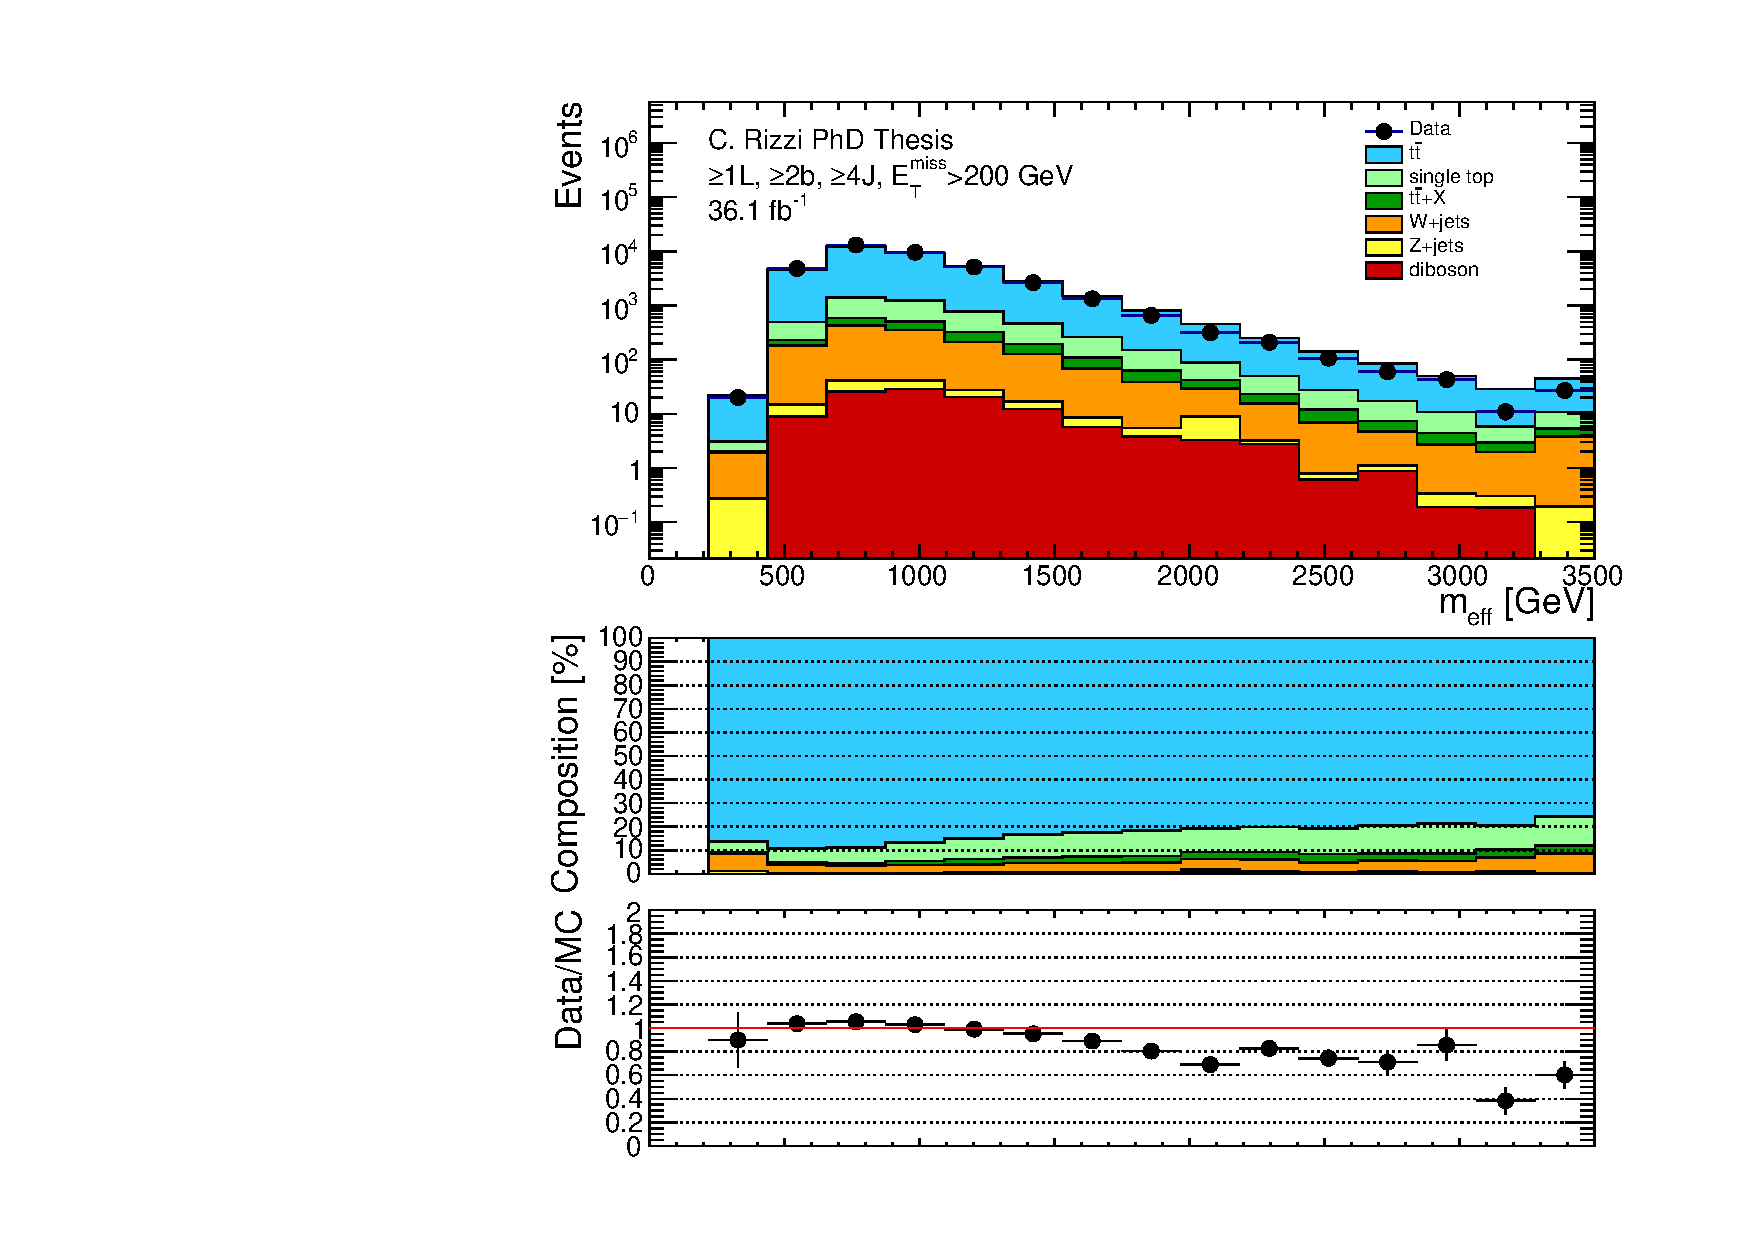
\includegraphics[width=0.49\textwidth]{figures/strong_prod/data_mc/1L_2bin/data_mc_meff_incl.pdf}
\label{fig:strong:datamc:meff_prerw_1L}}
\subfigure[]{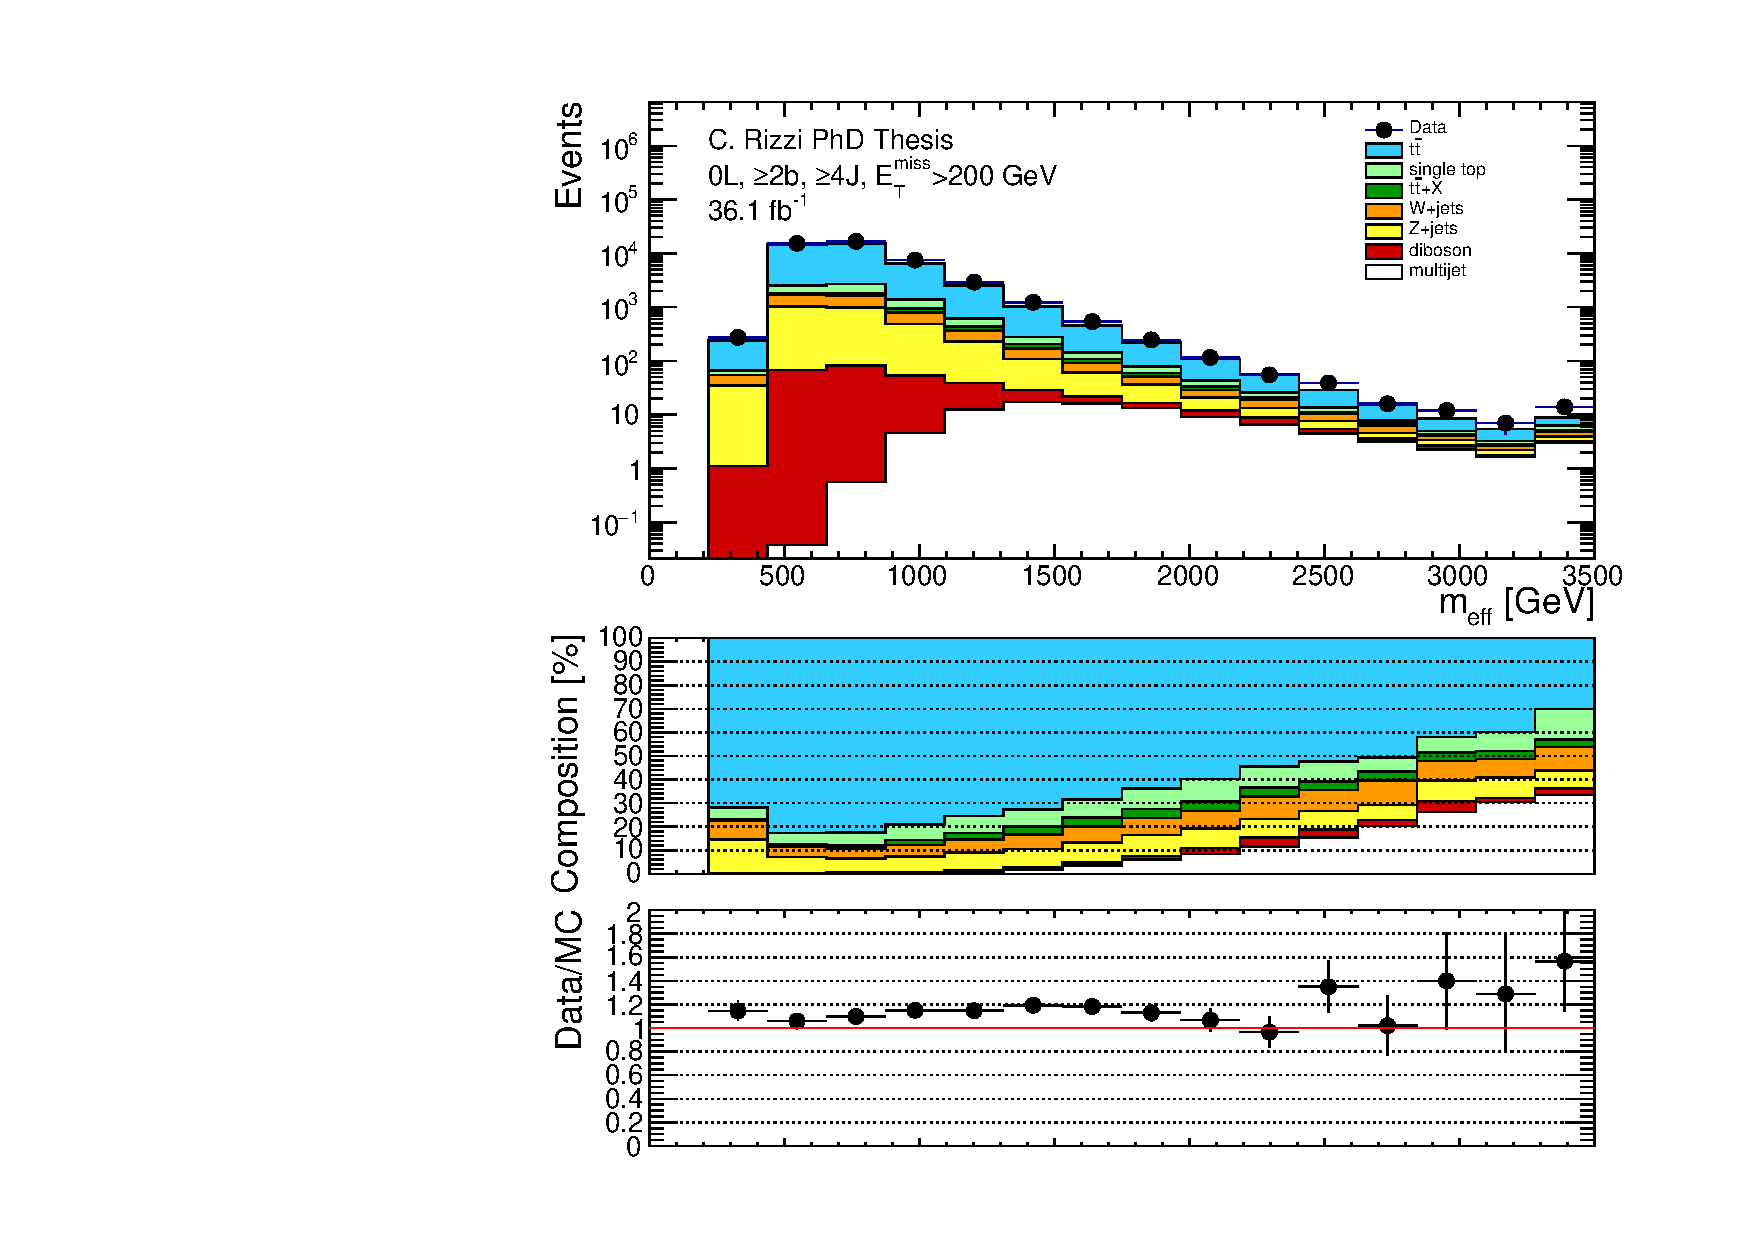
\includegraphics[width=0.49\textwidth]{figures/strong_prod/data_mc/0L_2bin/data_mc_meff_incl.pdf}
\label{fig:strong:datamc:meff_prerw_0L}}
\caption{ \subref{fig:strong:datamc:meff_prerw_1L}
}
\label{fig:strong:datamc:meff_prerw}
\end{figure*}

While the downward trend in the data/MC ratio in the 1-lepton channel is clearly visible in the bottom panel of Figure \ref{fig:strong:datamc:meff_prerw_1L},
Figure \ref{fig:strong:datamc:meff_prerw_0L} shows that this is not present in the 0-lepton channel.
This difference in trends is problematic for the analysis, since all of the \glspl{vr} require at least one signal lepton, 
including the ones used to derive the prediction for 0-lepton \glspl{sr}. 

To mitigate this problem and to have a better estimate of the background in the high-\meff tail, a reweighting is derived 
based on the distribution of \meff in a region that requires exactly two b-jets and low \mtb and is therefore
 orthogonal to all the analysis regions. More details on the reweighting procedure and on its validation are given in Appendix \ref{app:meffrw}.
All the plots in the rest of this section assume that the reweighting has already been applied. 


\subsection*{Data-MC comparison after the reweighting}


%data_mc_dphi_1jet.pdf
%data_mc_bjets_n.pdf
%data_mc_jets_n.pdf
%data_mc_pt_jet_1.pdf
%data_mc_dphi_min.pdf


\begin{figure*}[h]
\centering 
\subfigure[\meff]{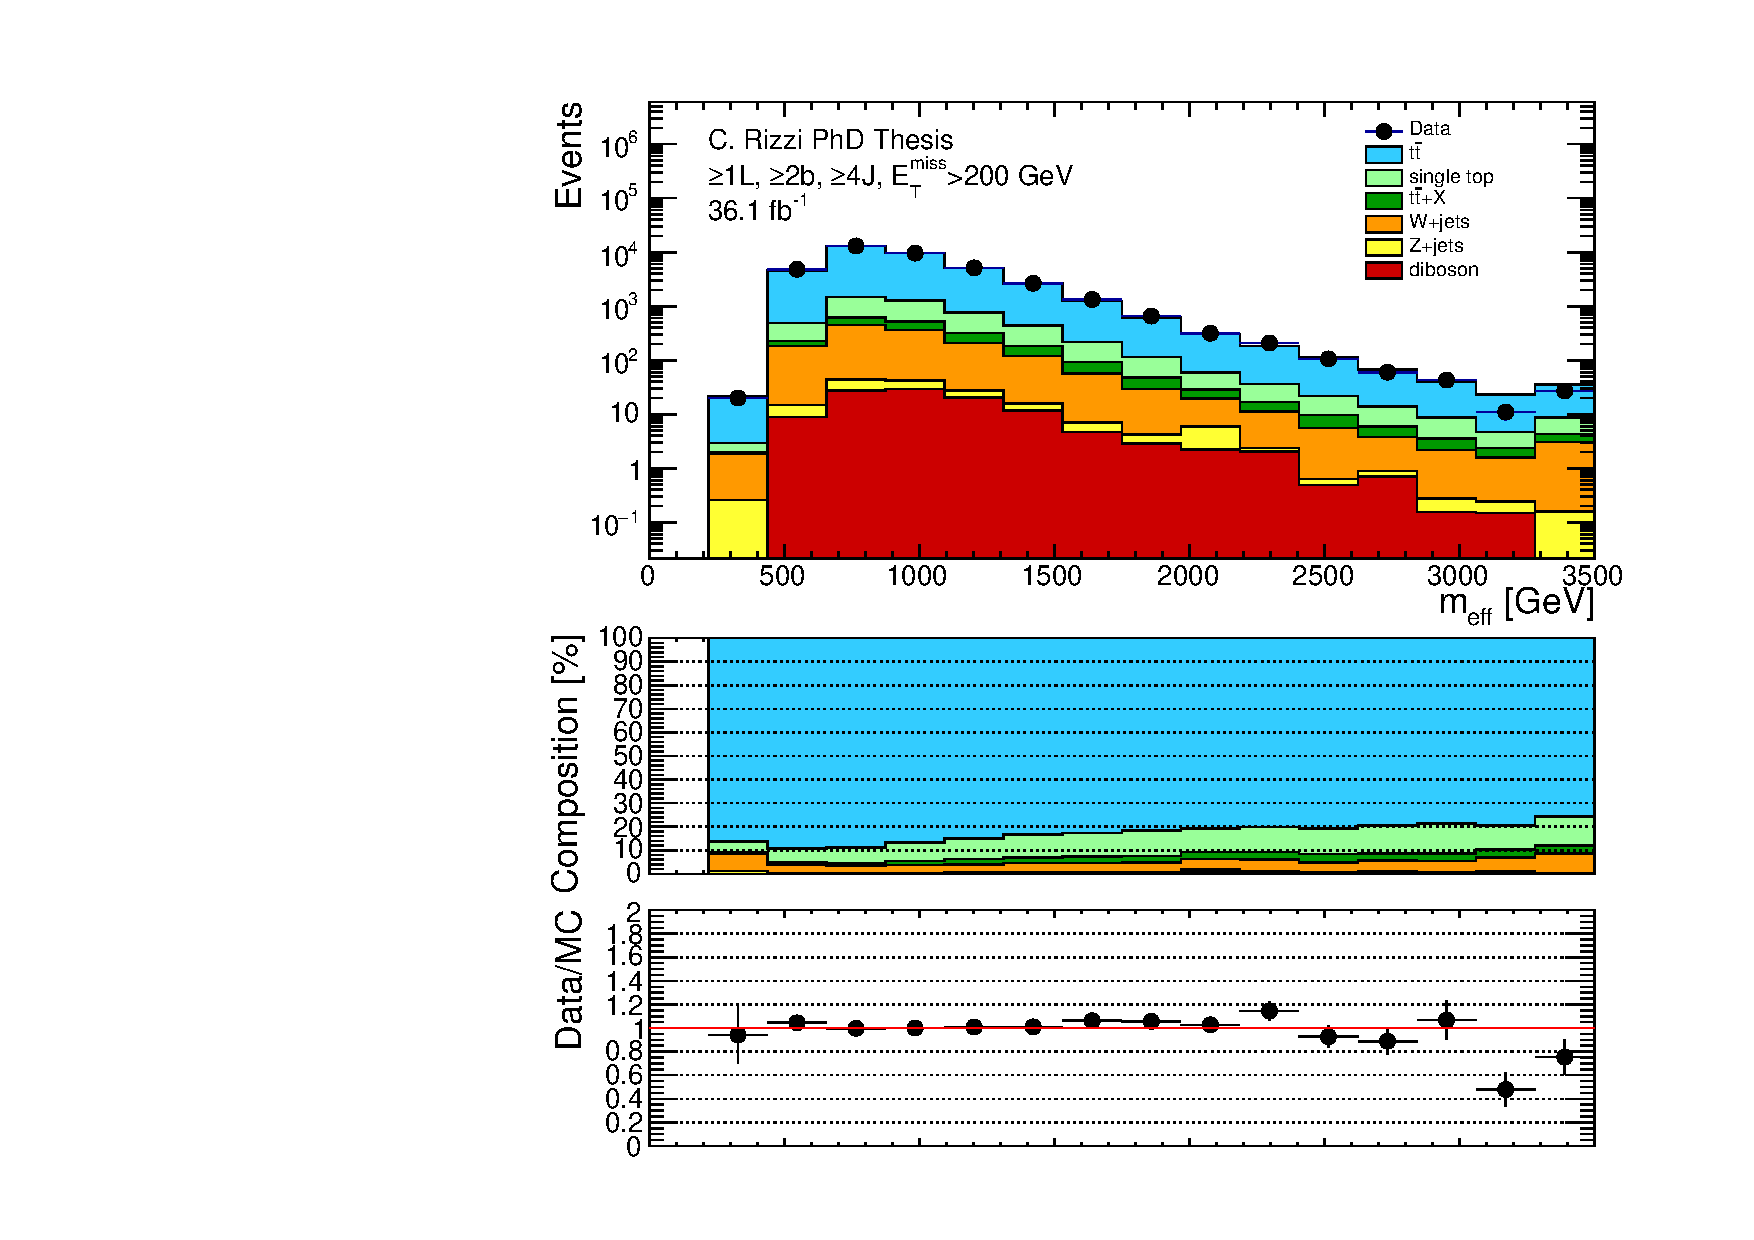
\includegraphics[width=0.45\textwidth]{figures/strong_prod/data_mc/1L_2bin_rw/data_mc_meff_incl.pdf}
\label{fig:strong:datamc1L:meff_incl}}
\subfigure[\mjsum]{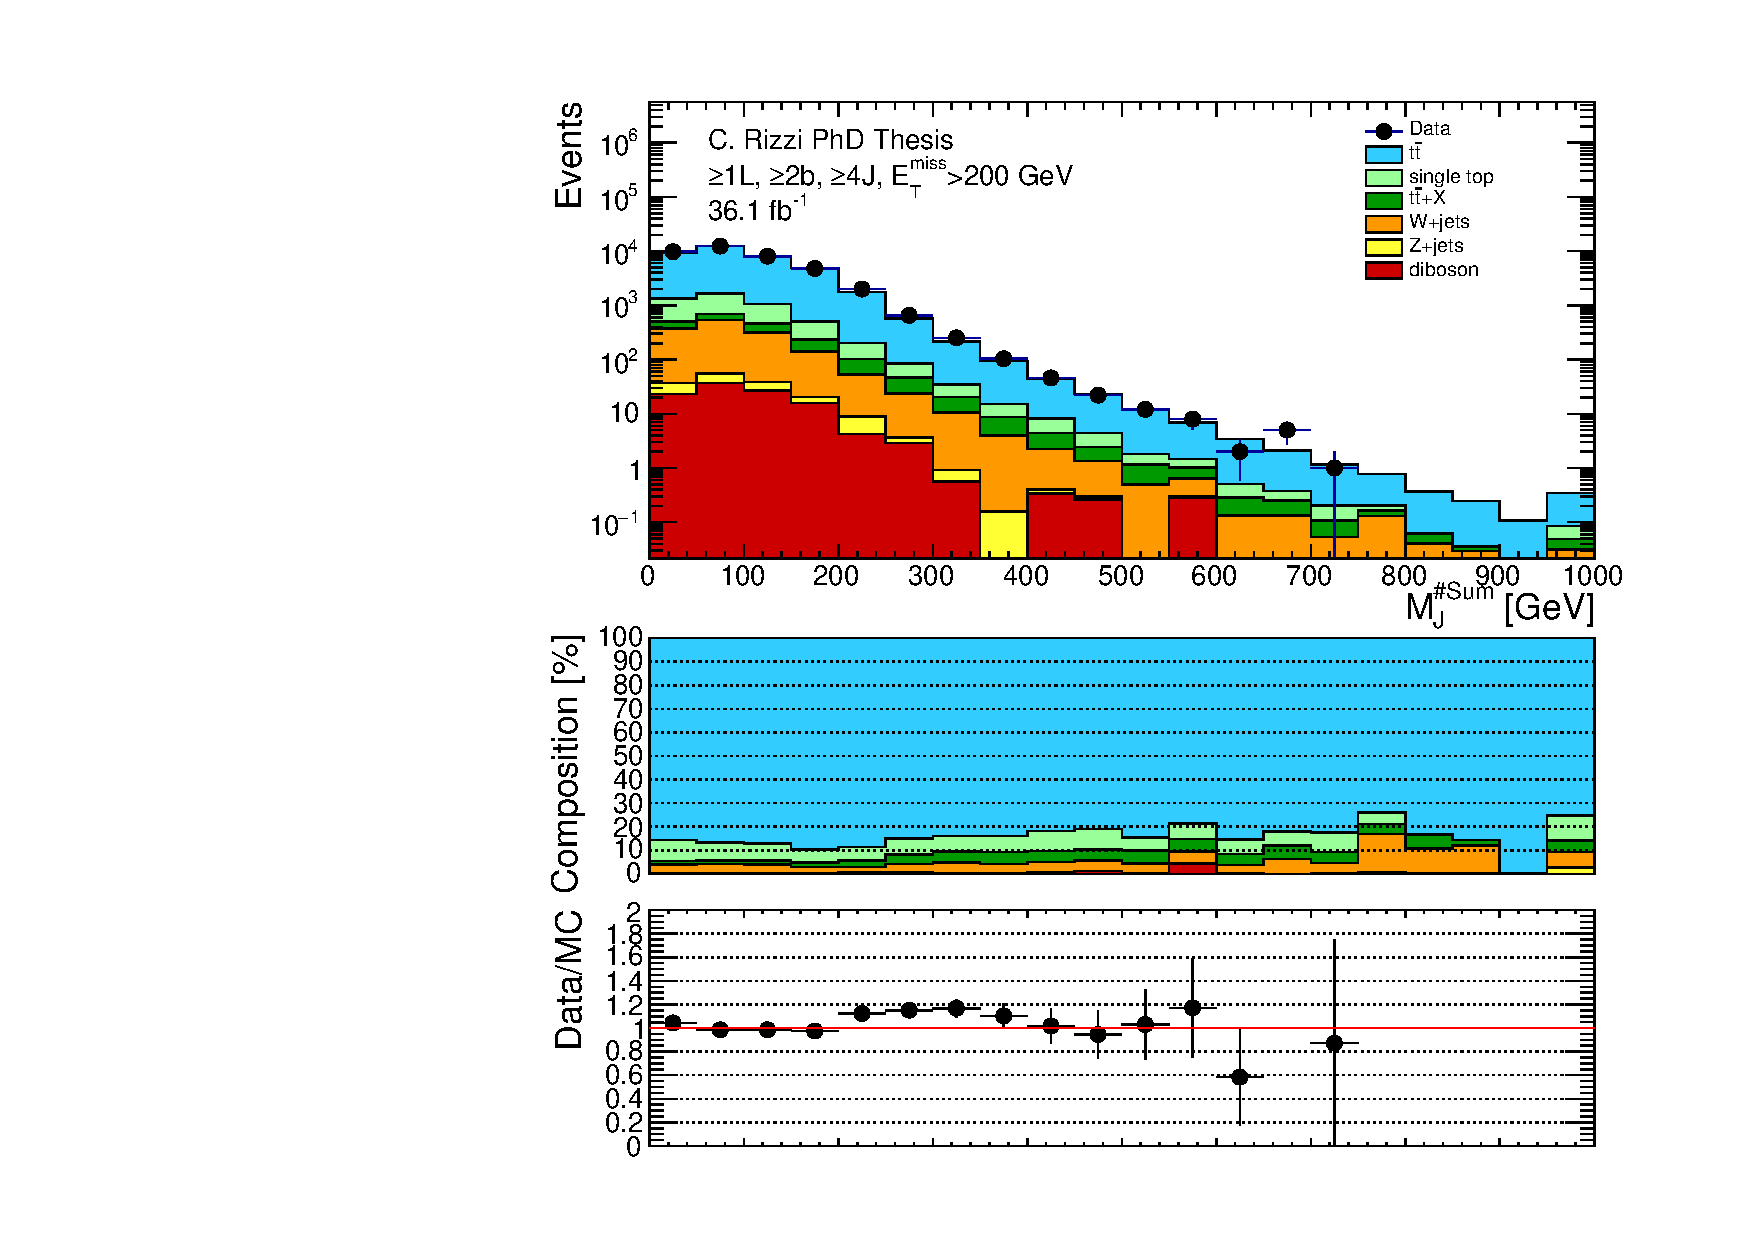
\includegraphics[width=0.45\textwidth]{figures/strong_prod/data_mc/1L_2bin_rw/data_mc_MJSum_rc_r08pt10.pdf}
\label{fig:strong:datamc1L:MJSum_rc_r08pt10}}\\
\subfigure[\met]{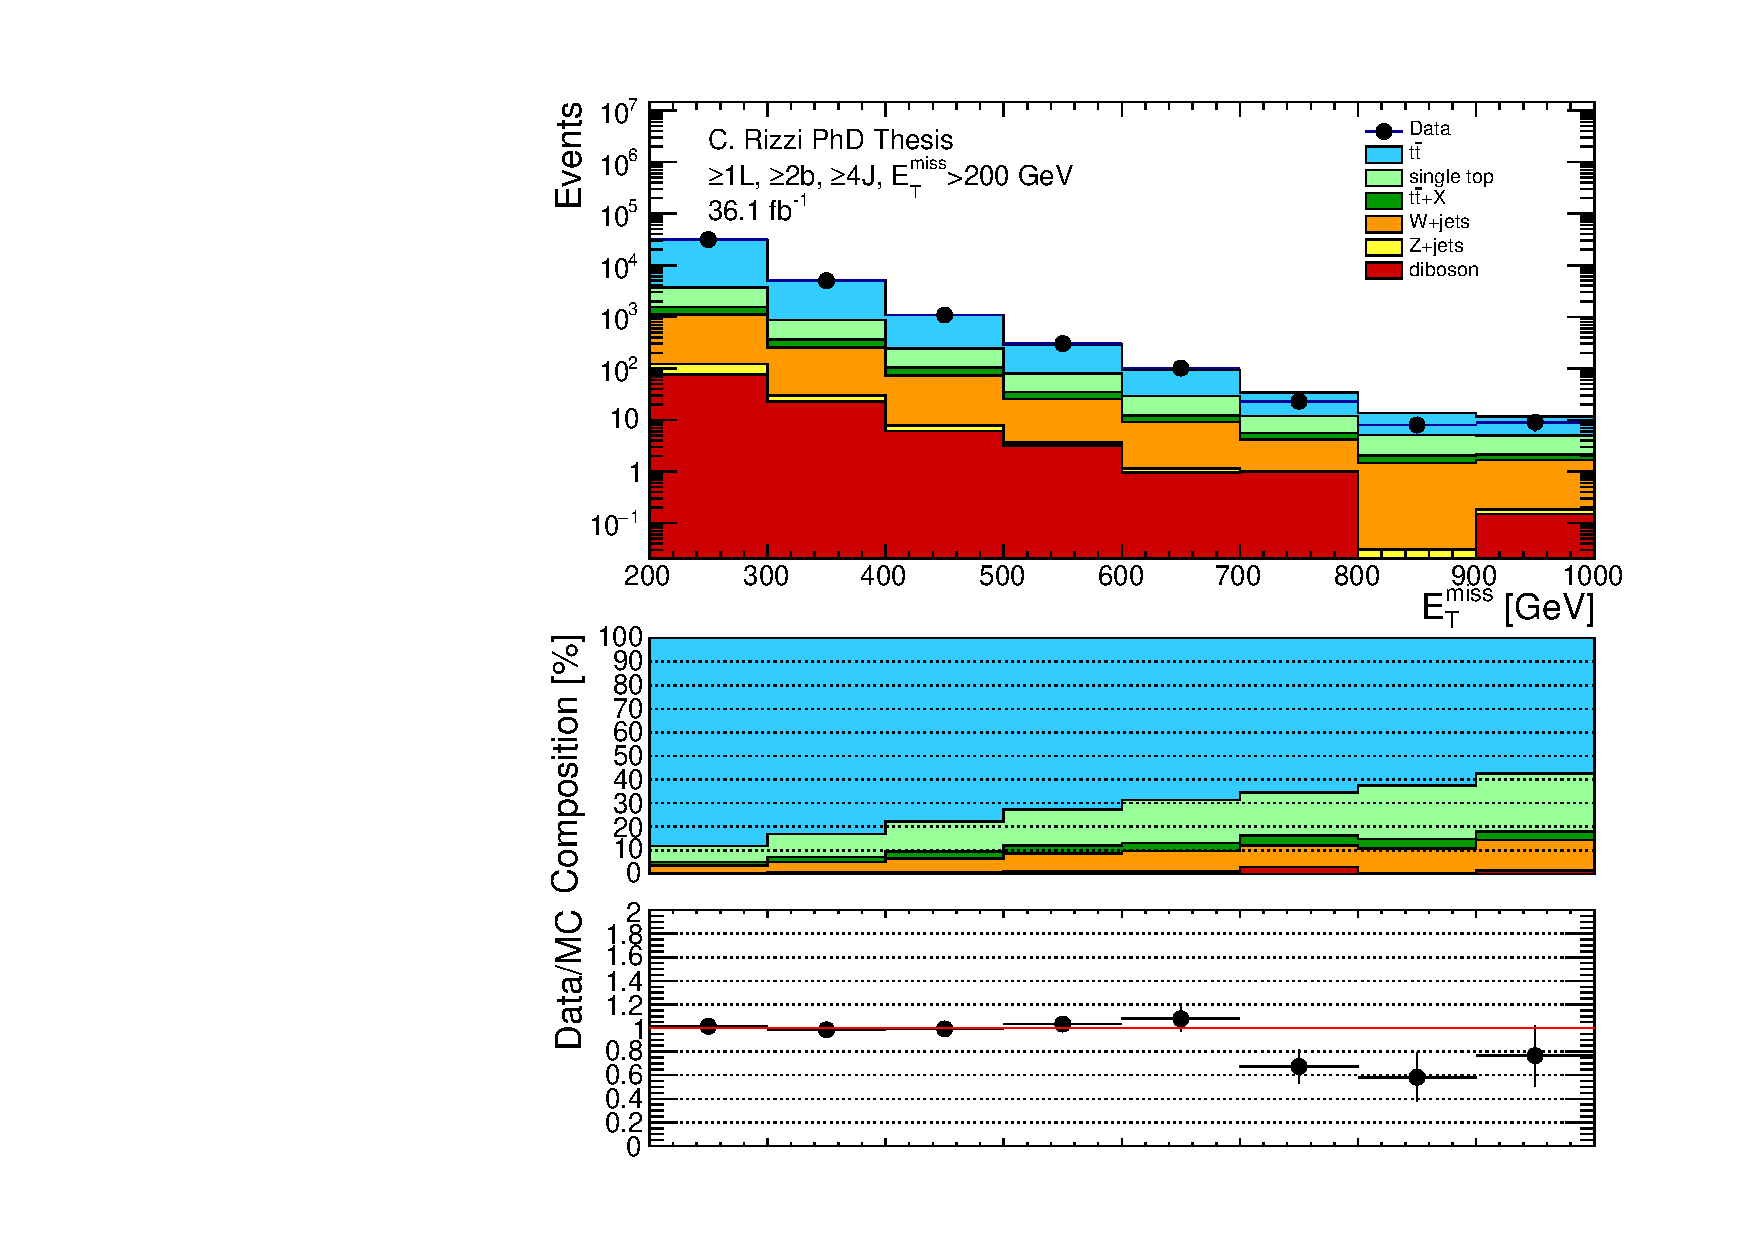
\includegraphics[width=0.45\textwidth]{figures/strong_prod/data_mc/1L_2bin_rw/data_mc_met.pdf}
\label{fig:strong:datamc1L:met}}
\subfigure[$\phi$(\met)]{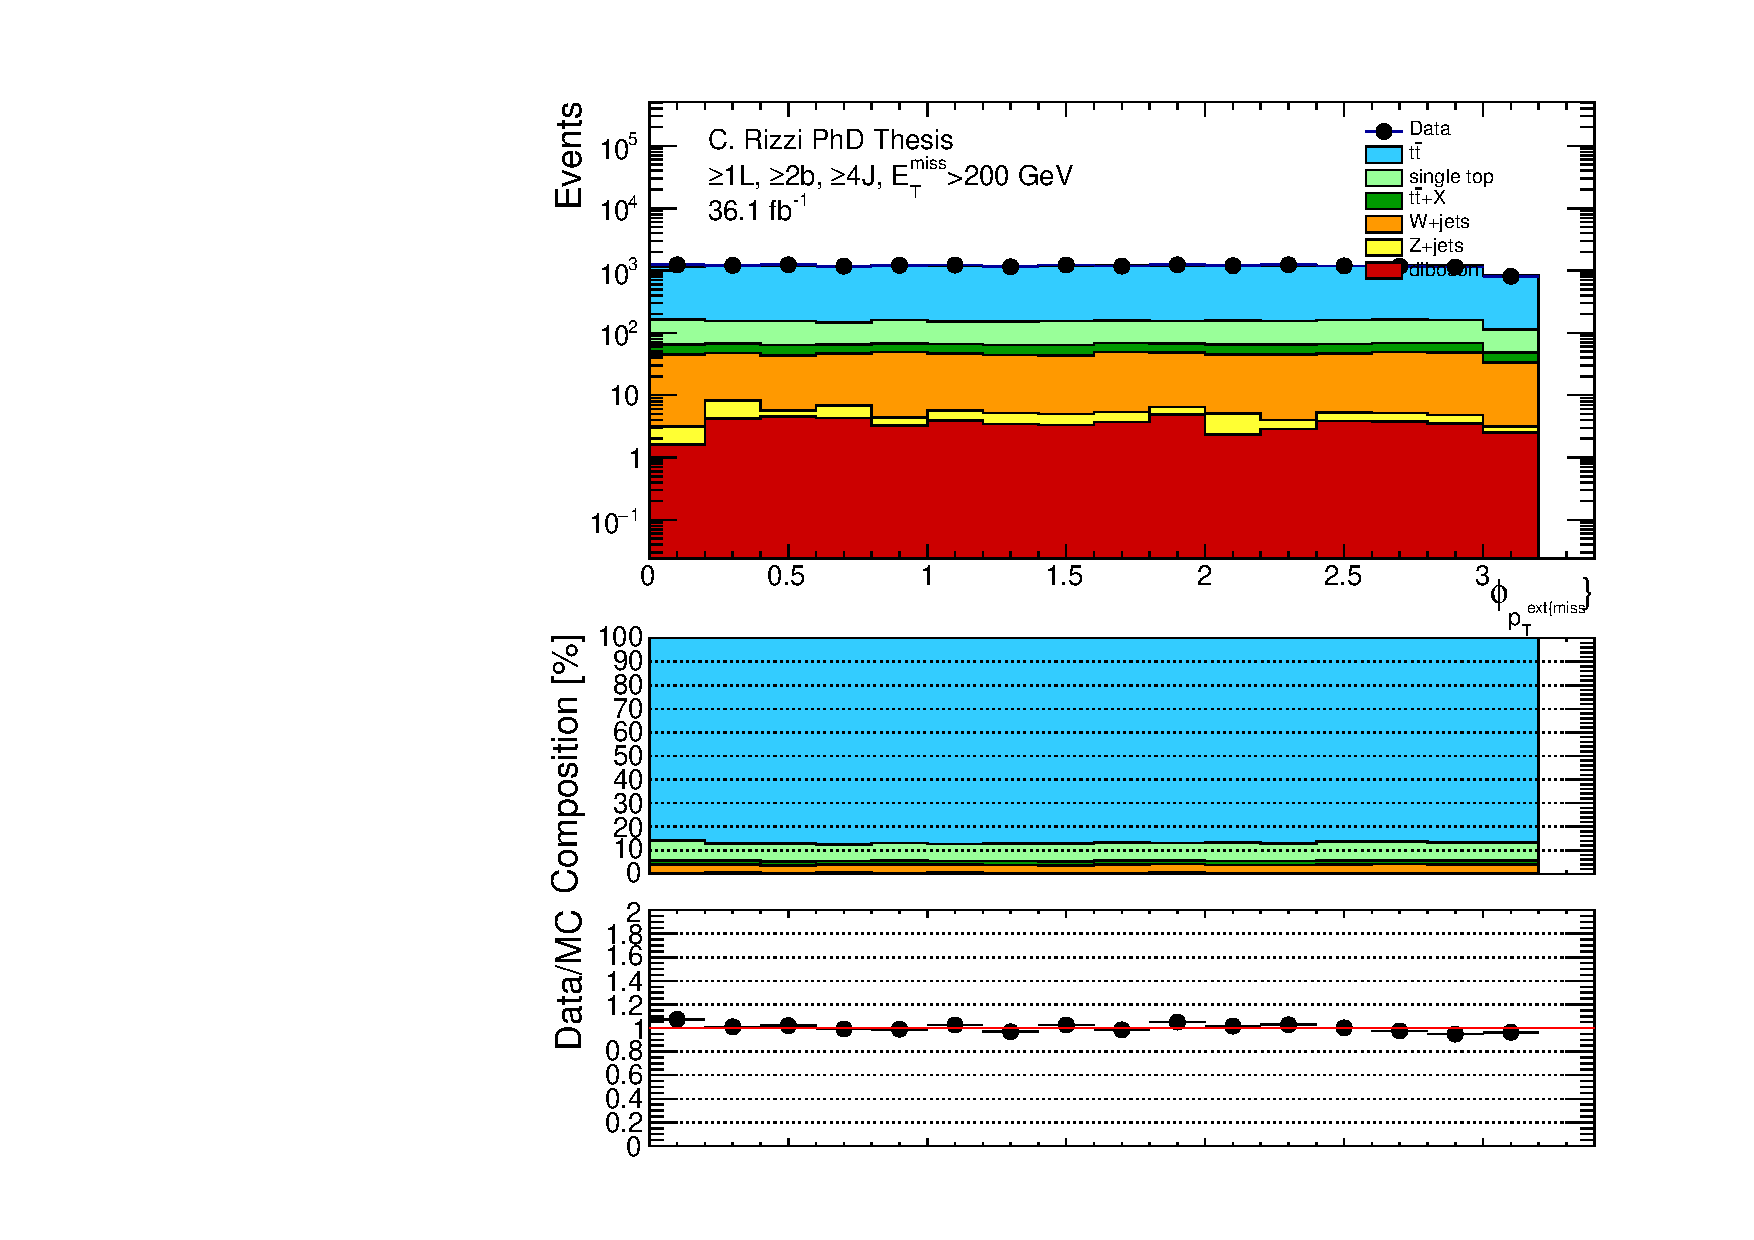
\includegraphics[width=0.45\textwidth]{figures/strong_prod/data_mc/1L_2bin_rw/data_mc_met_phi.pdf}
\label{fig:strong:datamc1L:met_phi}}\\
\subfigure[\mt]{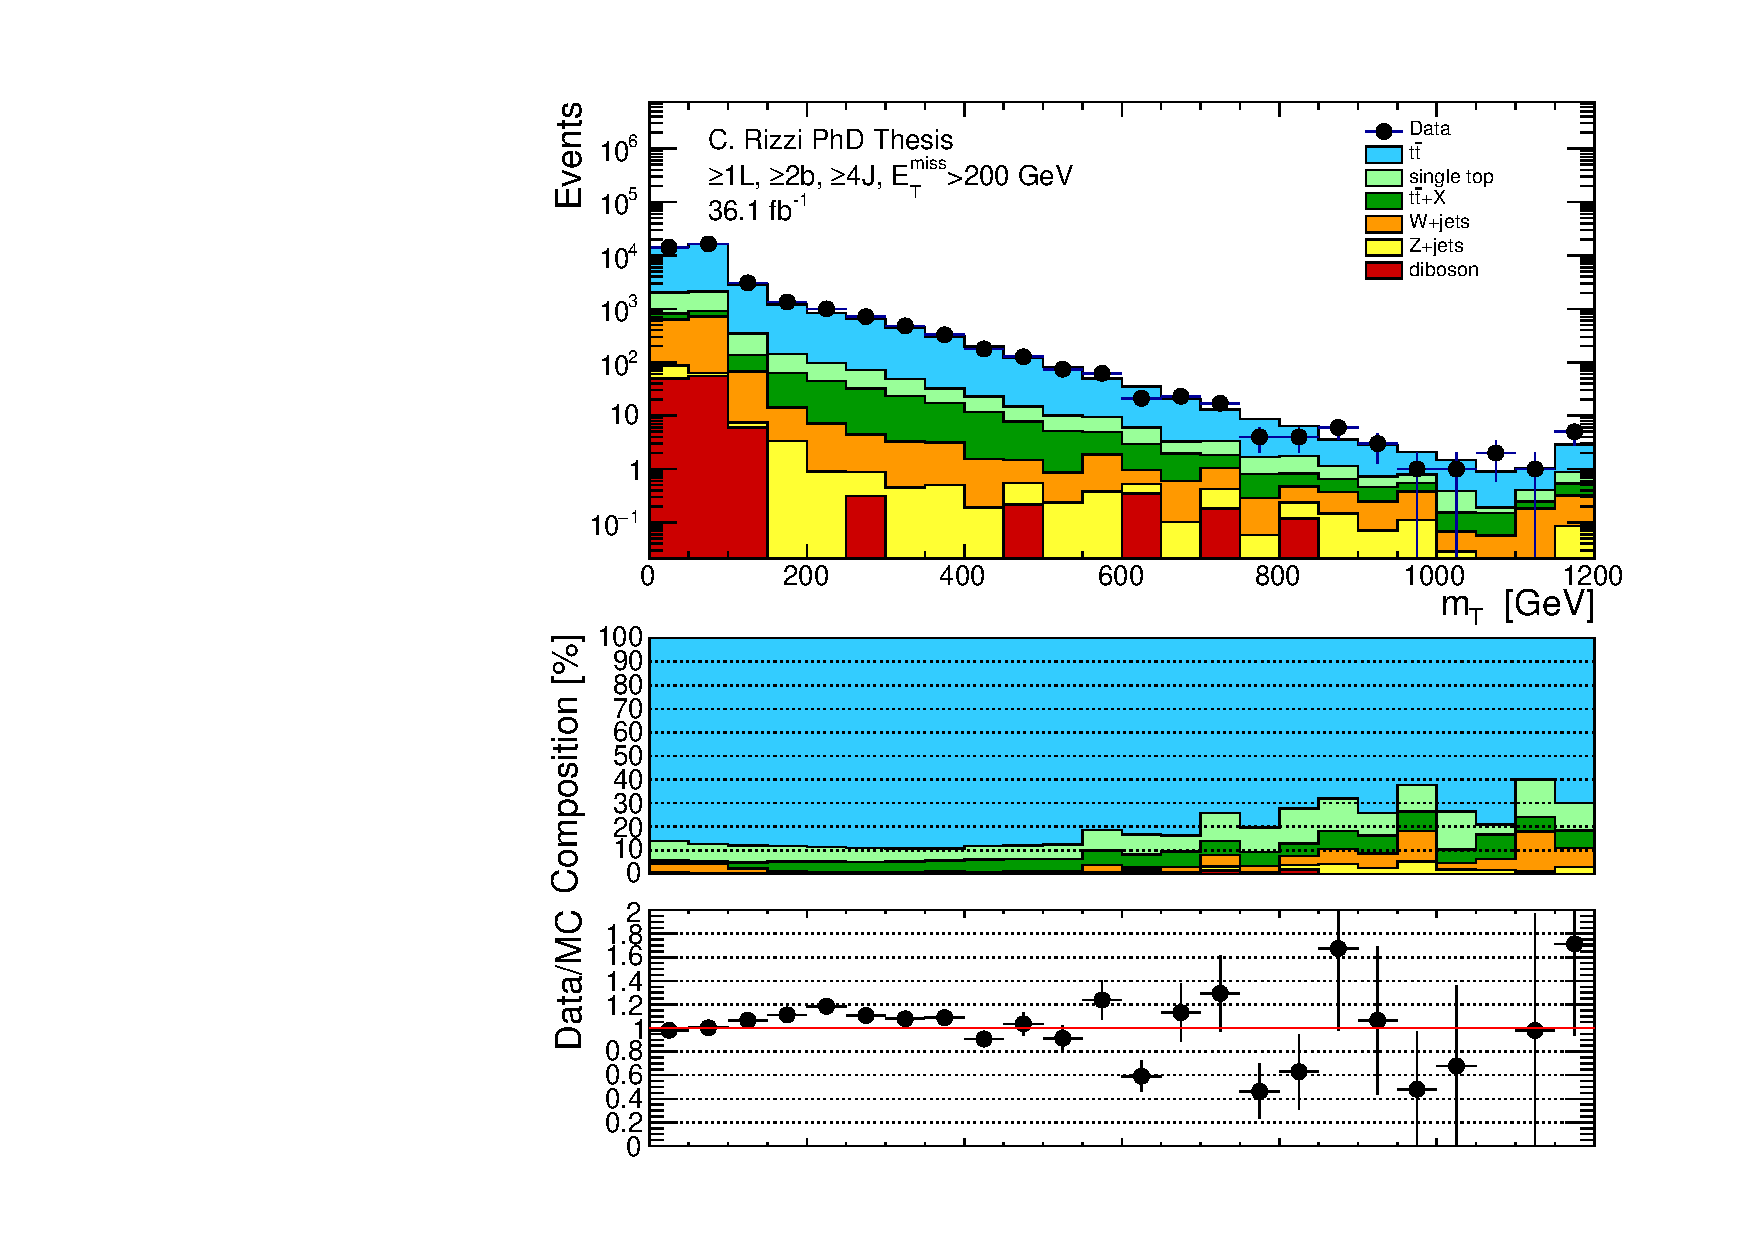
\includegraphics[width=0.45\textwidth]{figures/strong_prod/data_mc/1L_2bin_rw/data_mc_mT.pdf}
\label{fig:strong:datamc1L:mT}}
\subfigure[\mtb]{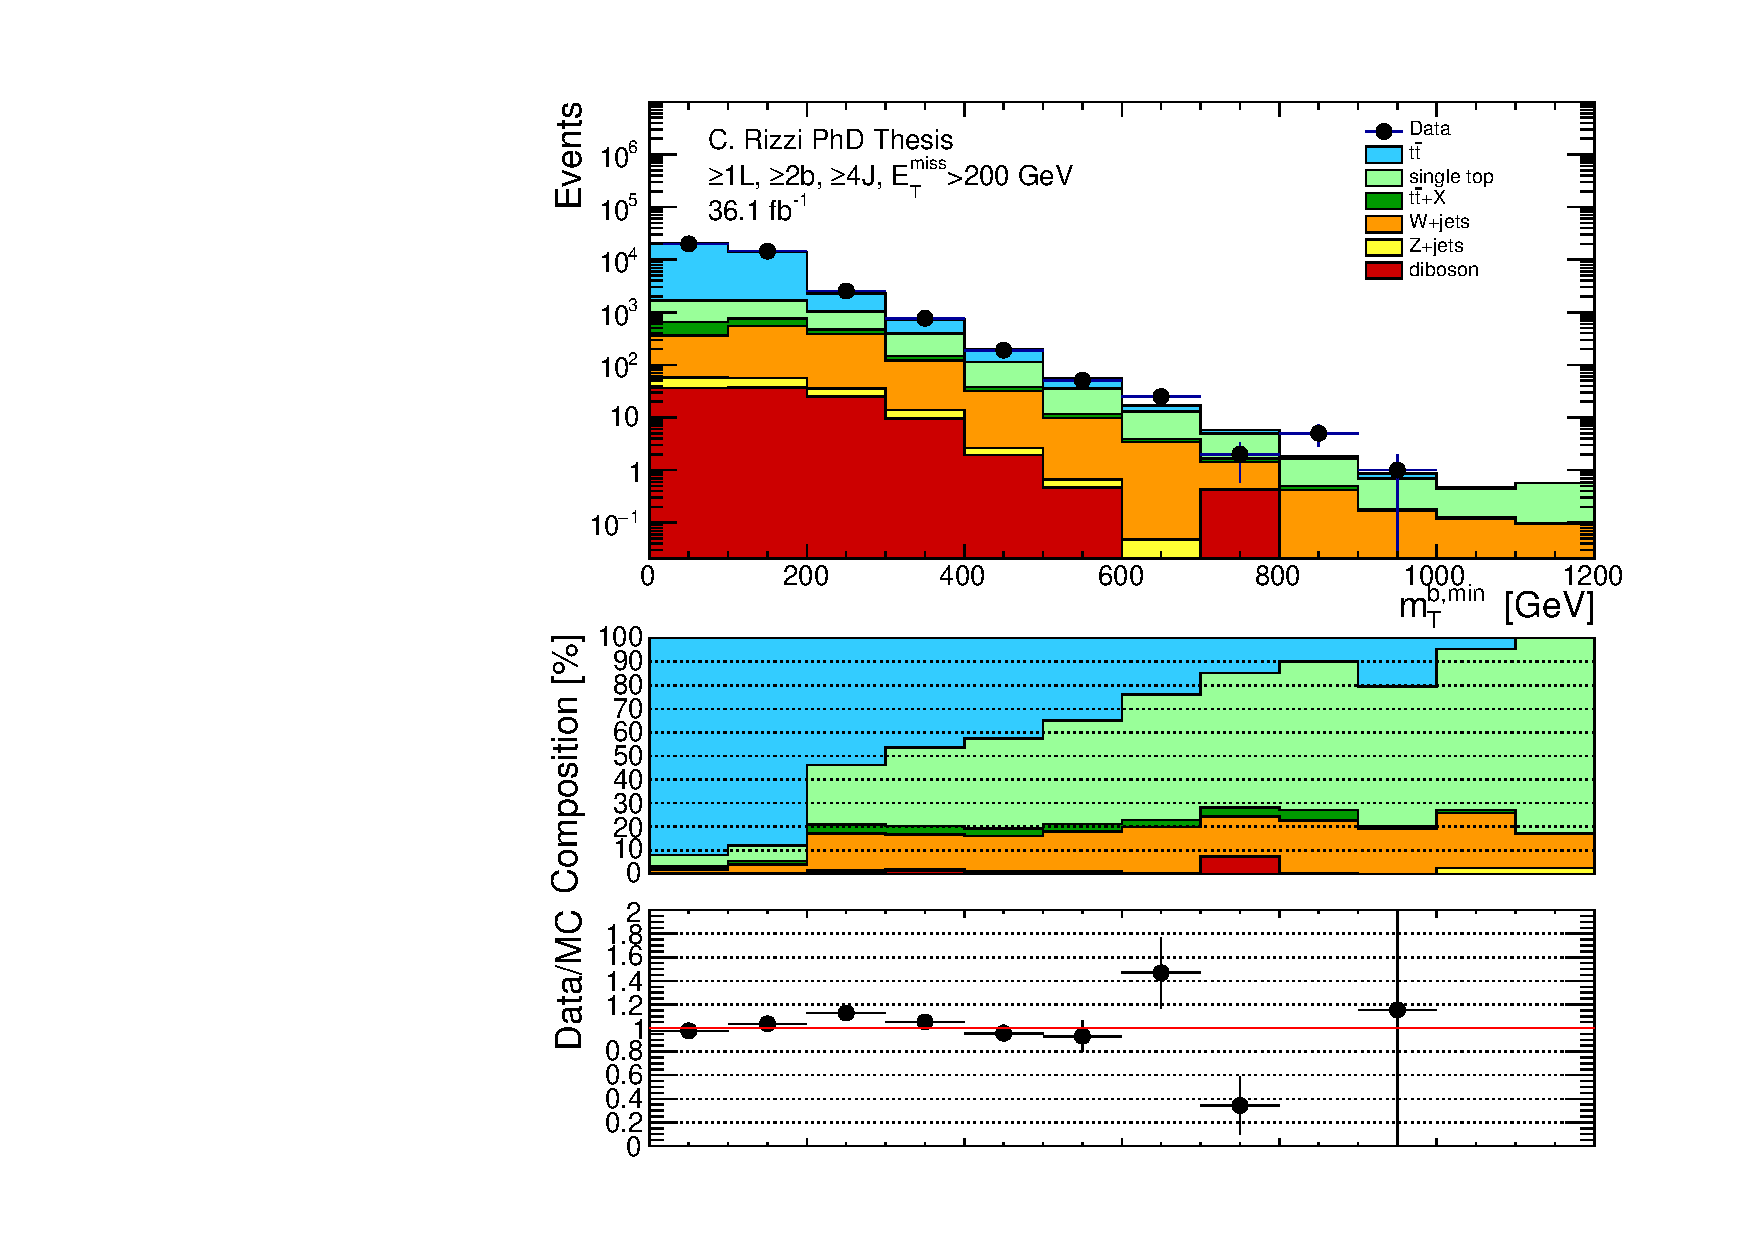
\includegraphics[width=0.45\textwidth]{figures/strong_prod/data_mc/1L_2bin_rw/data_mc_mTb_min.pdf}
\label{fig:strong:datamc1L:mTb_min}}
\caption{Data-MC comparison in the 1-lepton preselection, after applying the kinematic reweighting.
}
\label{fig:strong:datamc1L_a}
\end{figure*}


